\documentclass[../main.tex]{subfiles}
\begin{document}
	
\section{Simulation Evidence}
\label{sec:simulation}

The simulations examine how target-coefficient sensitivity arises, how influence localisation relates to estimation, and how similar sensitivity can emerge from model misspecification. The three studies address these questions sequentially. The first evaluates when conventional contamination outliers coincide with observations carrying substantial joint influence on the target slope. The second examines how localisation of those observations relates to post-deletion coefficient estimation and robust estimation. The third studies whether model misspecification can generate concentrated coefficient sensitivity without a planted contamination set. Algorithmic and calibration checks support these analyses and are reported separately where appropriate.

\subsection{Outlyingness and Target-Coefficient Influence}
\label{subsec:detection-performance}

The first simulation examines how conventional outlyingness aligns with target-coefficient influence under different contamination mechanisms. Response outliers, good leverage, and bad leverage generate distinct relationships between sample unusualness and target-slope movement. Classical diagnostics rank observations using residual extremeness, leverage, or single-observation influence, while fixed-\(k\) MIS searches jointly for the size-\(k\) set that maximises target-coefficient movement. Recovery of the injected set therefore measures how closely each contamination mechanism aligns contamination status with joint target-coefficient influence.

\begin{figure}[htbp]
	\centering
	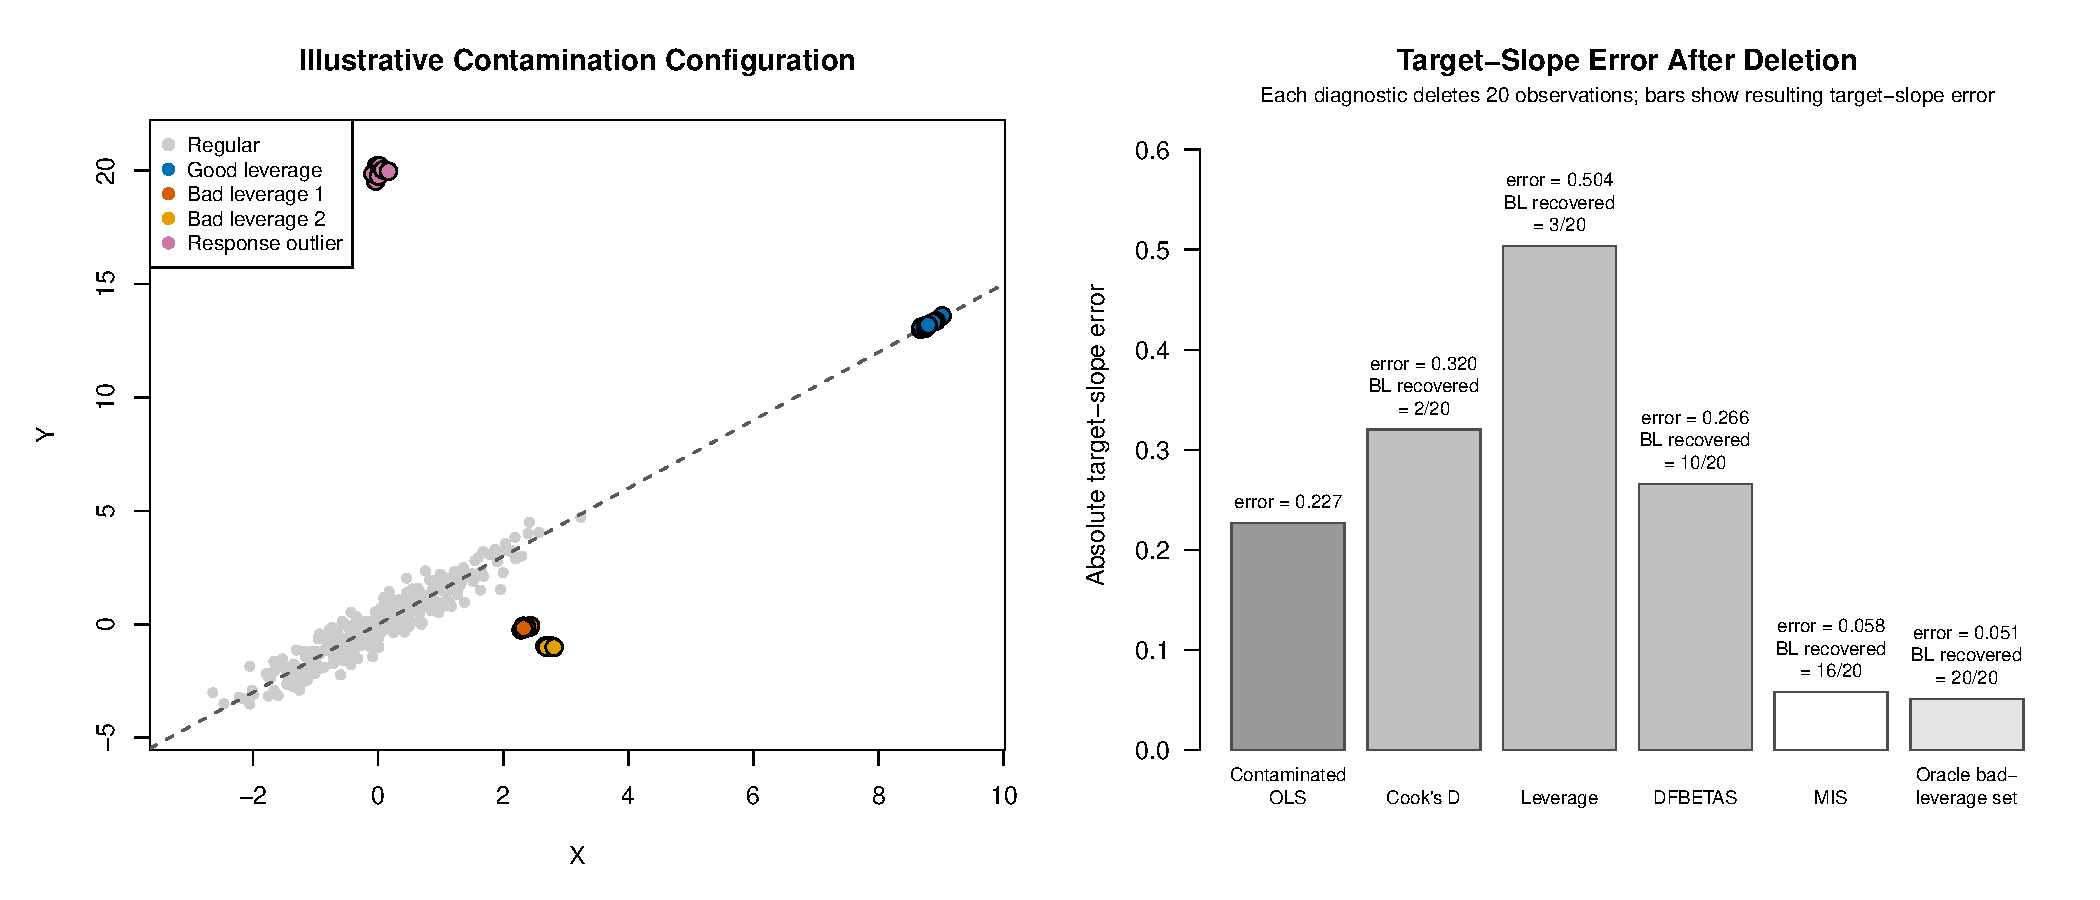
\includegraphics[width=\linewidth]{../../output/fig1_classical_vs_mis_demo.pdf}
	\caption{Deterministic conceptual demonstration of joint target-slope influence under a bad-leverage configuration. The figure contrasts visually unusual observations, single-observation diagnostics, and fixed-\(k\) MIS, illustrating a masking-like failure of casewise diagnostics. The coefficient comparison reports absolute target-slope error; contaminated OLS provides the undeleted baseline, while the deletion methods remove 20 observations.}
	\label{fig:classical-vs-mis-demo}
\end{figure}

The design varies sample size \(n\in\{500,1000,2500,5000\}\) and contamination proportion \(c\in\{0.005,0.01,0.025,0.05,0.10\}\). The injected-set size is
\[
k=\max\{\lfloor cn\rfloor,2\}.
\]
The simulation therefore supplies oracle \(k\). For contaminated samples, the known injected set is also used to resolve the directional ambiguity of the fixed-\(k\) search. Observation identities are not supplied to the subsequent search itself. The resulting procedure is therefore an oracle-assisted localisation benchmark for both set size and direction. It is referred to below as MIS with oracle \(k\) and oracle direction.

The three contamination mechanisms differ in how they affect the target slope. Response outliers shift the outcome at ordinary covariate positions, while good-leverage observations move far into predictor space but remain approximately aligned with the regression relation. Bad leverage combines both features: high leverage is paired with a response shift that rotates the fitted slope. All methods are evaluated against the same injected set.

Bad leverage produces the strongest alignment between contamination status and target-coefficient influence. In the equal-weight design-cell summary, MIS recovered \(92.9\%\) of the injected observations, compared with \(86.5\%\) for the highest-recovery classical diagnostic (\autoref{tab:02-detection-power-summary}). Across the sample-size--contamination grid, the target-aware recovery difference remained positive and ranged from \(8.0\) to \(16.0\) percentage points (\autoref{fig:02-mis-advantage}). \autoref{tab:02-detection-power-summary} uses the highest classical recovery throughout, whereas the figure uses the lowest classical benchmark for the two negative-control mechanisms. The bad-leverage design therefore shows close correspondence between the planted contamination mechanism and the set carrying the greatest target-slope influence.

\begin{table}[htbp]
\centering
\caption{Injected-set recovery and MIS-EVT rejection across contaminated designs. Each entry gives equal weight to the recorded design-cell summaries. The classical recovery benchmark is the highest recovery among Cook's D, leverage, and DFBETAS within each design cell before averaging.}
\label{tab:02-detection-power-summary}
\resizebox{\columnwidth}{!}{%
\begin{tabular}{@{}lrrrr@{}}
\toprule
Contamination mechanism & MIS recovery & Highest classical recovery & MIS-EVT rejection & EVT convergence \\
\midrule
Response outliers & 26.6\% & 48.4\% & 42.6\% & 99.7\% \\
Good leverage & 36.9\% & 70.1\% & 1.6\% & 99.7\% \\
Bad leverage & 92.9\% & 86.5\% & 91.9\% & 99.7\% \\
\bottomrule
\end{tabular}%
}
\end{table}


\begin{figure}[htbp]
	\centering
	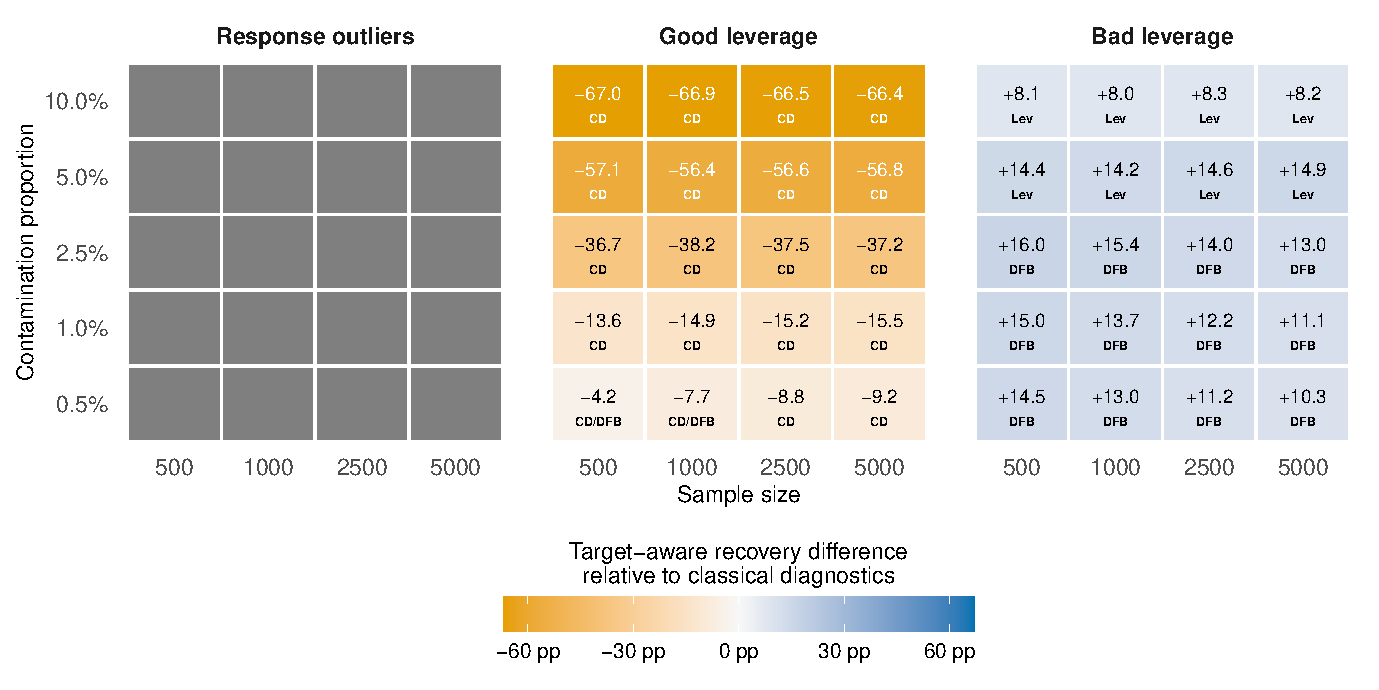
\includegraphics[width=\linewidth]{../../output/02_distributional/figures/main/02_fig1_mis_advantage_heatmap.pdf}
	\caption{Target-aware recovery difference between MIS and classical diagnostics across sample sizes, contamination proportions, and contamination mechanisms. For bad leverage, the benchmark is the highest-recovery classical diagnostic and positive values indicate greater recovery by MIS. For response outliers and good leverage, the benchmark is the lowest-recovery classical diagnostic and positive values indicate lower unnecessary recovery by MIS. The cell label identifies the classical diagnostic defining the benchmark.}
	\label{fig:02-mis-advantage}
\end{figure}

Response outliers produce substantially weaker alignment between contamination status and target-slope influence. MIS recovered \(26.6\%\) of the injected observations, compared with \(48.4\%\) for the highest-recovery classical diagnostic (\autoref{tab:02-detection-power-summary}). Classical procedures can identify these observations through their residual extremeness, while the MIS objective depends on their contribution to target-coefficient movement. Large residuals therefore need not correspond to large joint influence on the target slope.

Good leverage produces an even larger separation between covariate extremeness and target-slope influence. The highest-recovery classical diagnostic recovered \(70.1\%\) of the injected observations, while MIS recovered \(36.9\%\) (\autoref{tab:02-detection-power-summary}). The injected observations occupy extreme predictor positions but remain approximately aligned with the fitted relation. Their covariate extremeness therefore carries relatively limited information about their joint influence on the target slope. The mechanism diagnostic below examines this separation directly.

A separate mechanism diagnostic examines this result at \(n=1000\), \(k=10\), with normal predictors and \(200\) Monte Carlo iterations per error distribution. MIS-selected observations typically had much lower leverage but substantially larger residual and absolute-DFBETA magnitudes than the injected good-leverage set (\autoref{fig:02-good-leverage-mechanism} and \autoref{tab:02-good-leverage-mechanism}). Under normal errors, for example, the median leverage ratio was \(0.07\), while the corresponding absolute-DFBETA and residual ratios were \(19.19\) and \(131.91\). The diagnostic therefore tracks coefficient influence more closely than covariate extremeness.

\begin{figure}[htbp]
	\centering
	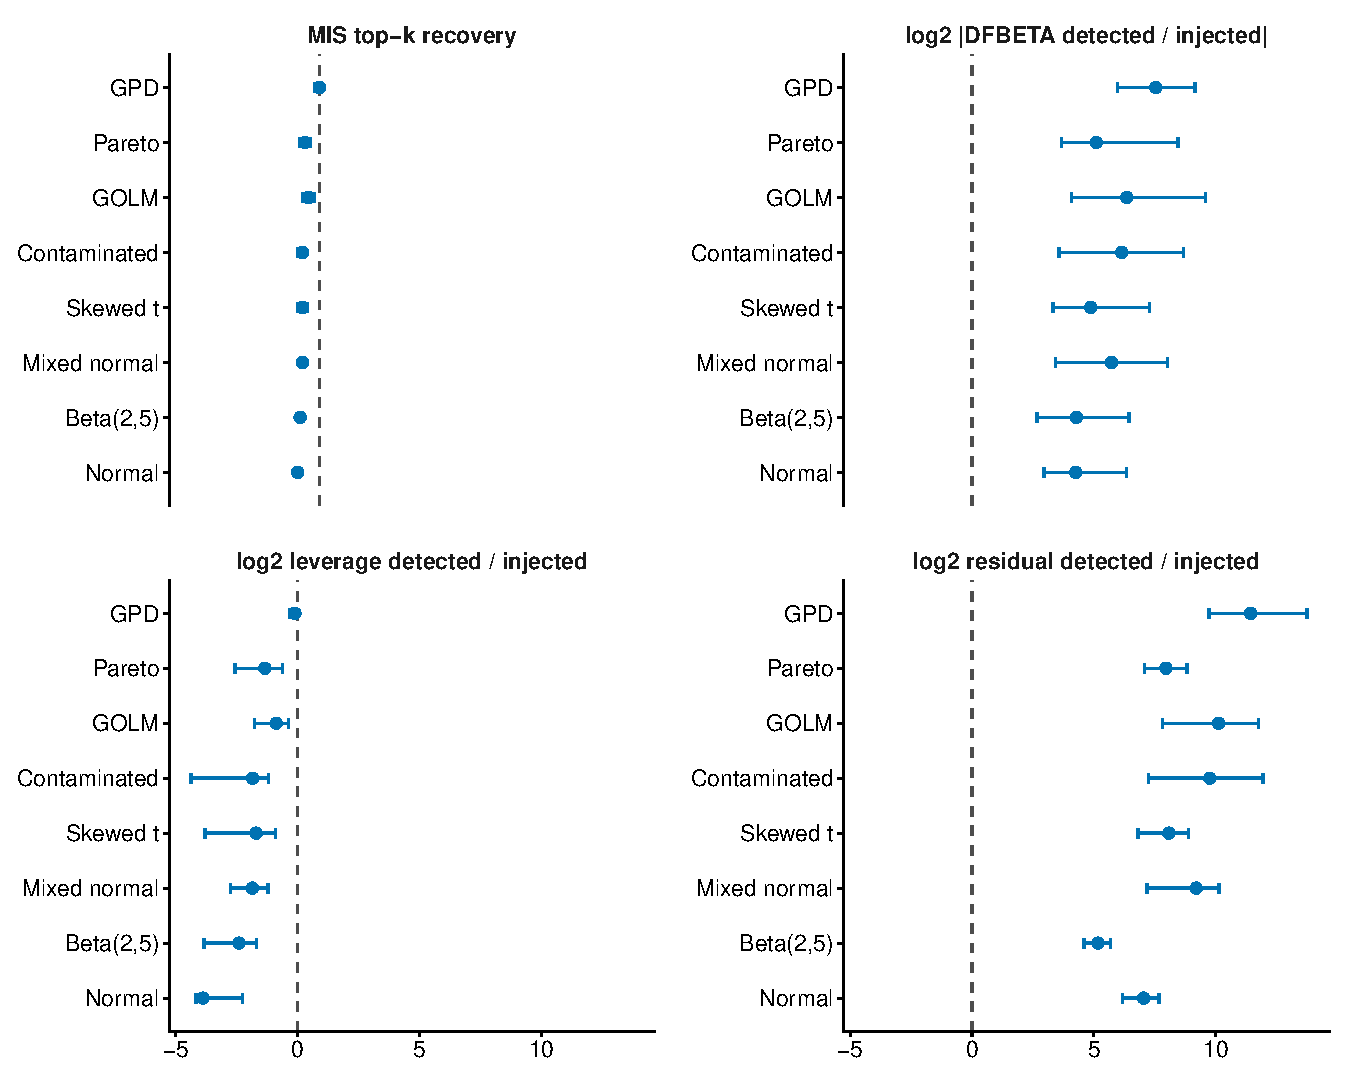
\includegraphics[width=0.92\linewidth]{../../output/02_distributional/figures/main/02_fig3_good_leverage_mechanism.pdf}
	\caption{Good-leverage mechanism diagnostics by error distribution. The MIS recovery panel reports injected-set top-\(k\) recovery. The remaining panels compare absolute DFBETA, leverage, and residual magnitude between the MIS-selected and injected sets on a base-two logarithmic ratio scale; zero denotes equality.}
	\label{fig:02-good-leverage-mechanism}
\end{figure}

\begin{table}[htbp]
\centering
\caption{Good-leverage mechanism diagnostic by error distribution. Entries are medians with 10th--90th percentile intervals; ratios compare the MIS-selected set with the injected set.}
\label{tab:02-good-leverage-mechanism}
\resizebox{\columnwidth}{!}{%
\begin{tabular}{@{}lrrrr@{}}
\toprule
Error distribution & MIS recovery & Absolute DFBETA ratio & Leverage ratio & Residual ratio \\
\midrule
Normal & 0.0\% [0.0, 10.0] & 19.19 [7.79, 81.13] & 0.07 [0.06, 0.21] & 131.91 [72.50, 204.94] \\
Beta(2,5) & 10.0\% [0.0, 20.0] & 19.49 [6.34, 87.44] & 0.19 [0.07, 0.31] & 36.07 [24.17, 51.22] \\
Mixed normal & 20.0\% [10.0, 30.0] & 52.84 [10.70, 257.82] & 0.28 [0.15, 0.43] & 587.85 [145.26, 1129.02] \\
Skewed t & 20.0\% [0.0, 40.0] & 29.29 [10.04, 155.03] & 0.31 [0.07, 0.53] & 269.58 [111.79, 470.79] \\
Contaminated & 20.0\% [0.0, 30.0] & 70.83 [11.91, 410.78] & 0.28 [0.05, 0.44] & 865.07 [150.41, 3942.18] \\
GOLM & 45.0\% [20.0, 70.0] & 81.67 [17.04, 765.92] & 0.54 [0.29, 0.78] & 1110.72 [225.44, 3455.62] \\
Pareto & 30.0\% [10.0, 51.0] & 34.24 [12.81, 349.75] & 0.39 [0.17, 0.65] & 248.45 [135.75, 454.45] \\
GPD & 90.0\% [70.0, 90.0] & 186.35 [63.06, 565.51] & 0.92 [0.79, 0.94] & 2769.74 [845.42, 13780.70] \\
\bottomrule
\end{tabular}%
}
\end{table}


The mechanism-dependent recovery pattern remains stable across most of the recorded error distributions. Under bad leverage, MIS recovery exceeded \(97\%\) for normal, Beta\((2,5)\), mixed-normal, skewed-\(t\), and Pareto errors, but fell to \(78.5\%\) under GPD errors (\autoref{fig:02-distributional-robustness}). The simulated GPD shape parameters are \(\xi\in\{1.5,3,5,10\}\), for which the population mean does not exist. This condition serves as an extreme stress design. Auxiliary MIS-EVT calibration and block-count diagnostics are reported in \autoref{app:detection-results}, with the block-size restriction derived in \autoref{app:deriv-blocks}. Within the GPD stress design, the block-maxima calibration deteriorates sharply as the deletion fraction increases and becomes fully degenerate at \(2.5\%\) and above.

\begin{figure}[htbp]
	\centering
	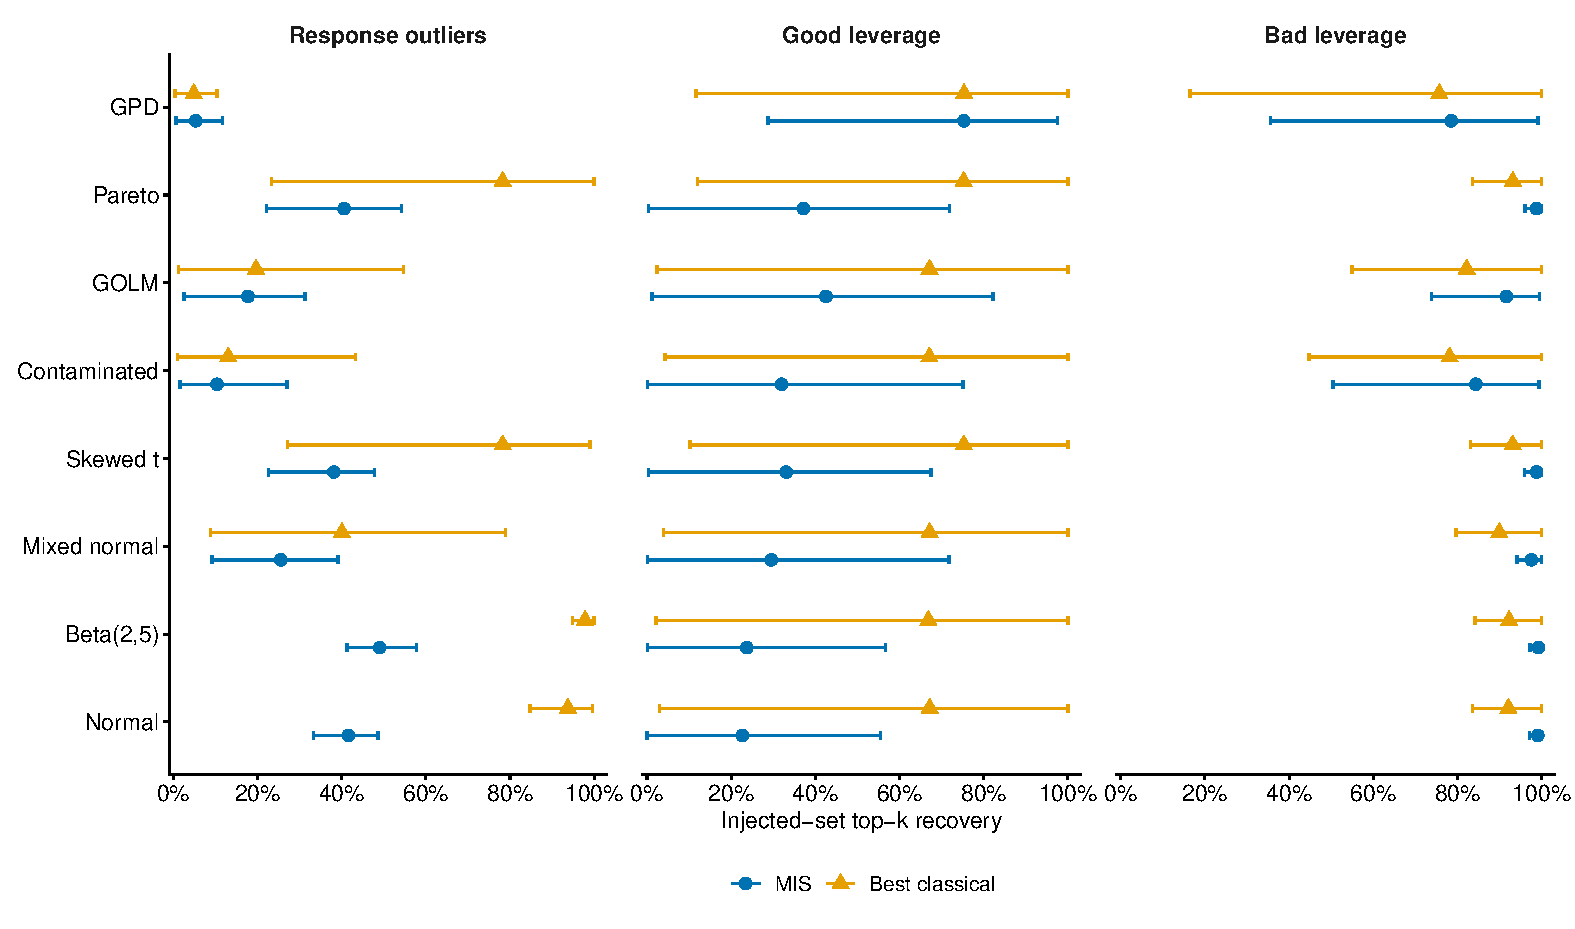
\includegraphics[width=\linewidth]{../../output/02_distributional/figures/main/02_fig2_distributional_robustness.pdf}
	\caption{Distributional robustness of injected-set top-\(k\) recovery for MIS and the highest-recovery classical diagnostic. Points report mean recovery across the recorded design cells, and intervals report the corresponding 10th--90th percentile range.}
	\label{fig:02-distributional-robustness}
\end{figure}


The three contamination mechanisms show that alignment between outlyingness and target-coefficient influence depends on how the contamination process affects the target slope. Bad leverage produces close alignment because the planted observations jointly distort the coefficient, while response outliers and good leverage produce weaker alignment between sample unusualness and coefficient movement. Recovery of a planted set therefore has a mechanism-specific interpretation. The next simulation examines what localisation of coefficient influence implies for subsequent coefficient estimation.











\subsection{Influence Localisation and Estimation}
\label{subsec:estimation-performance}

The second simulation examines how influence localisation relates to coefficient estimation under contamination. Leverage, Cook's distance, DFBETAS, and fixed-\(k\) MIS select observations before an OLS refit. MM regression and LTS estimate the coefficient using resistant fitting rules. The comparison therefore separates two statistical objectives: locating observations that carry coefficient influence and stabilising coefficient estimation under contamination.

The design varies sample size \(n\in\{500,1000,2500,5000\}\), contamination proportion \(c\in\{0.005,0.01,0.025,0.05\}\), three predictor environments, and eight error distributions. The primary comparison uses the finite-moment design cells and treats the infinite-mean GPD condition separately as a stress case. MIS is evaluated as an oracle-assisted localisation benchmark: the search is supplied with the injected-set size \(k\) and the direction of the induced target-coefficient perturbation, while the identities of the injected observations remain unknown to the search. This isolates localisation conditional on the deletion budget and search direction. Under no contamination, oracle \(k=0\), so MIS coincides with full-sample OLS by construction.

\begin{figure}[htbp]
	\centering
	\includegraphics[width=\linewidth]{../../output/04_robust/figures/main/04_fig1_coefficient_error_distributions.pdf}
	\caption{Empirical distributions of signed target-coefficient error across methods and contamination mechanisms in the primary finite-moment designs. Monte Carlo draws are shown on a signed pseudo-logarithmic scale; filled circles denote arithmetic means and open diamonds denote medians. Separation between the two summaries can indicate asymmetry or the influence of infrequent large coefficient errors on average performance.}
	\label{fig:04-coefficient-errors}
\end{figure}

The coefficient-error distributions distinguish typical Monte Carlo performance from average performance. The median describes the centre of each simulated error distribution, while the arithmetic mean responds more strongly to asymmetry and infrequent large errors. Separation between the two markers therefore identifies settings in which typical coefficient error and average coefficient error convey different performance patterns. The full distributions make this tail behaviour visible alongside the summary statistics. The infinite-mean GPD design is treated separately as a stress condition.

The estimation consequences of localisation depend on whether the injected observations themselves drive target-coefficient distortion. Under response-outlier and good-leverage contamination, the injected observations can be unusual while exerting limited influence on the target slope. Conditional on oracle \(k\), MIS selects the size-\(k\) set that maximises coefficient movement, so the subsequent OLS refit can move a coefficient that was already close to its target value. Bad leverage produces a different relationship because the injected set itself generates substantial target-slope distortion. Localisation and post-deletion coefficient accuracy are therefore most closely aligned when the contamination mechanism also drives coefficient error.

MM regression and LTS produce more concentrated coefficient-error distributions because they directly modify the estimation rule under contamination. Fixed-\(k\) MIS solves a localisation problem by identifying a size-\(k\) set with large joint influence on the prespecified coefficient, conditional here on oracle \(k\) and direction. Localisation performance and estimator stability therefore describe separate performance dimensions. A method can achieve coefficient stability without identifying the set that maximises the fixed-\(k\) deletion objective.

The second simulation gives influence localisation a specific interpretation. Fixed-\(k\) MIS characterises where joint target-coefficient sensitivity is concentrated, while MM regression and LTS characterise coefficient stability under contamination. The mean--median differences in \autoref{fig:04-coefficient-errors} additionally show that typical and average Monte Carlo performance can diverge when coefficient-error distributions are asymmetric or contain infrequent large errors. These findings separate the structure of coefficient sensitivity from the performance of the resulting estimator. The final simulation examines whether concentrated coefficient sensitivity can also arise from model misspecification without a planted contamination set.



\subsection{Misspecification and Concentrated Coefficient Sensitivity}
\label{subsec:misspecification}

The third simulation examines whether model misspecification can generate concentrated coefficient sensitivity without a planted contamination set. Eight mechanisms are considered: linear endogeneity, nonlinear confounding, heterogeneous slopes, heteroskedasticity, a missing interaction, nonlinear functional form, an omitted variable, and threshold behaviour. Each mechanism is evaluated across \(96\) environments formed by four sample sizes, three predictor distributions, and eight error distributions. The design therefore broadens the source of target-coefficient sensitivity from injected observations to departures between the fitted specification and the data-generating process.

Fixed-\(k\) MIS is evaluated at deletion fractions \(k/n\in\{0.01,0.025,0.05,0.10\}\), with \(k/n=0.025\) used as the primary operating point. The MIS search produces one size-\(k\) candidate set in each coefficient direction under the fixed-residualised objective described in \autoref{sec:methodology}. Both candidates are then evaluated by full-refit validation, and \(S_k\) denotes the candidate producing the larger absolute movement in the refitted target coefficient. Target-coefficient sensitivity is summarised by
\[
T_k
=
\frac{
	\left|
	\widehat{\beta}_{-S_k}-\widehat{\beta}
	\right|
}{
	\widehat{\operatorname{se}}(\widehat{\beta})
},
\]
The statistic \(T_k\) measures full-refit coefficient movement in standard-error units. Here, \(\widehat{\beta}_{-S_k}\) is the full-refit target coefficient after deleting the selected set. Independent null simulations provide the reference distribution for \(T_k\). For each mechanism--environment combination, the detection boundary is the smallest simulated severity at which the fitted rejection probability reaches \(80\%\); combinations that do not reach this criterion within the simulated severity range are treated as right-censored. The remaining deletion fractions are treated as alternative sensitivity budgets rather than estimates of an underlying influential-set size.

The strength of concentrated coefficient sensitivity varies sharply across misspecification mechanisms. At the primary deletion fraction, nonlinear confounding, heterogeneous slopes, nonlinear functional form, and threshold behaviour reached the \(80\%\) detection criterion in all \(96\) environments, while the omitted-variable design reached it in \(8.3\%\) of environments. Linear endogeneity did not reach the criterion within the simulated severity range. The severity required to attain the criterion also differs across mechanisms. These patterns show that the form of misspecification determines whether coefficient sensitivity becomes strongly concentrated under the stated deletion budget.

\autoref{fig:05-boundary-by-n} shows how the severity required to attain the \(80\%\) criterion varies with sample size. For nonlinear confounding, heterogeneous slopes, missing interactions, nonlinear functional form, and threshold behaviour, the required severity generally falls as sample size increases. Heteroskedasticity shows the same pattern beyond the smallest design. Omitted-variable misspecification remains substantially weaker, while linear endogeneity does not attain the criterion within the simulated severity range.

\begin{figure}[htbp]
	\centering
	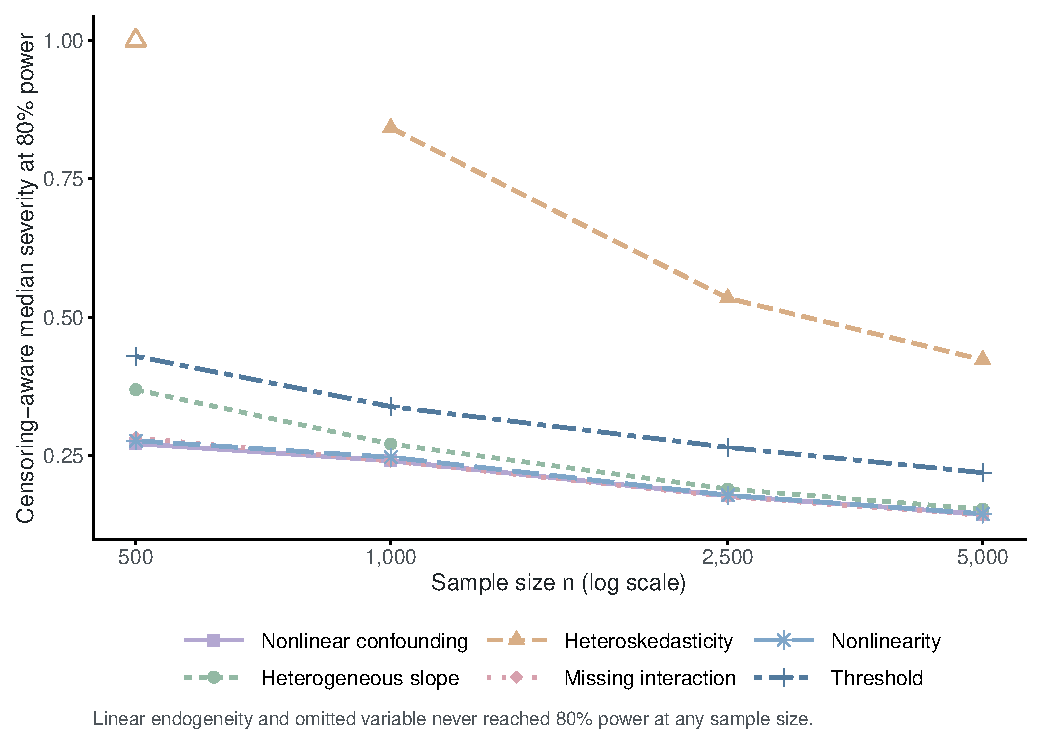
\includegraphics[width=0.82\linewidth]{../../output/05_misspecification/figures/main/05_fig03_boundary_by_n.pdf}
	\caption{Mechanism-dependent target-coefficient sensitivity of fixed-\(k\) MIS across sample sizes. Points report the censoring-aware median misspecification severity required to attain the \(80\%\) detection criterion. Mechanism--sample-size combinations that do not reach the criterion within the simulated severity range are treated as right-censored.}
	\label{fig:05-boundary-by-n}
\end{figure}

The deletion budget \(k\) remains a sensitivity parameter. Changing \(k/n\) changes the set over which influence is optimised and therefore changes the operating characteristics of the diagnostic. The simulated deletion fractions are interpreted as alternative fixed-budget sensitivity analyses; their relative performance does not identify a uniquely correct influential-set size.

Linear endogeneity provides an algebraic fitted-span invariance boundary case. In the simulated design, the endogeneity component lies within the fitted linear span, so increasing its severity changes the coefficient representation while leaving the relevant deletion-sensitivity structure unchanged. The MIS statistic is consequently invariant up to numerical precision across severity levels. Nonlinear confounding removes this fitted-span invariance and produces a strong response across the recorded environments. These two mechanisms show that misspecification can alter the target coefficient without necessarily concentrating its deletion sensitivity. Localisation then raises a further question: whether the observations selected by MIS correspond to a substantively defined affected subgroup. This comparison is available for the heterogeneous-slope and threshold designs.

The threshold design provides the clearest case. At \(k/n=0.025\), the MIS-selected set has precision \(0.606\) and lift \(2.43\) relative to an affected fraction of \(0.25\). Heterogeneous slopes produce a different pattern, with precision \(0.274\) and lift \(1.10\), close to the no-enrichment benchmark. A mechanism can therefore generate substantial target-coefficient sensitivity without causing the selected MIS observations to coincide closely with a nominal affected subgroup. Detection of coefficient sensitivity and localisation of a known subgroup are distinct properties.

Post-deletion refitting can leave the underlying misspecification unresolved and can increase coefficient error. The lower panels of \autoref{fig:05-targeting-localisation} show that coefficient RMSE can rise as the deletion budget grows after the selected observations are removed and the model is refitted. The relevant comparisons are within predictor environments because the panels use different vertical scales. Deletion changes the estimating sample, while model correction requires changes to the maintained specification or identifying assumptions. The result gives localisation a diagnostic interpretation: it identifies where finite-sample coefficient sensitivity is concentrated within the maintained specification.

\begin{figure}[htbp]
	\centering
	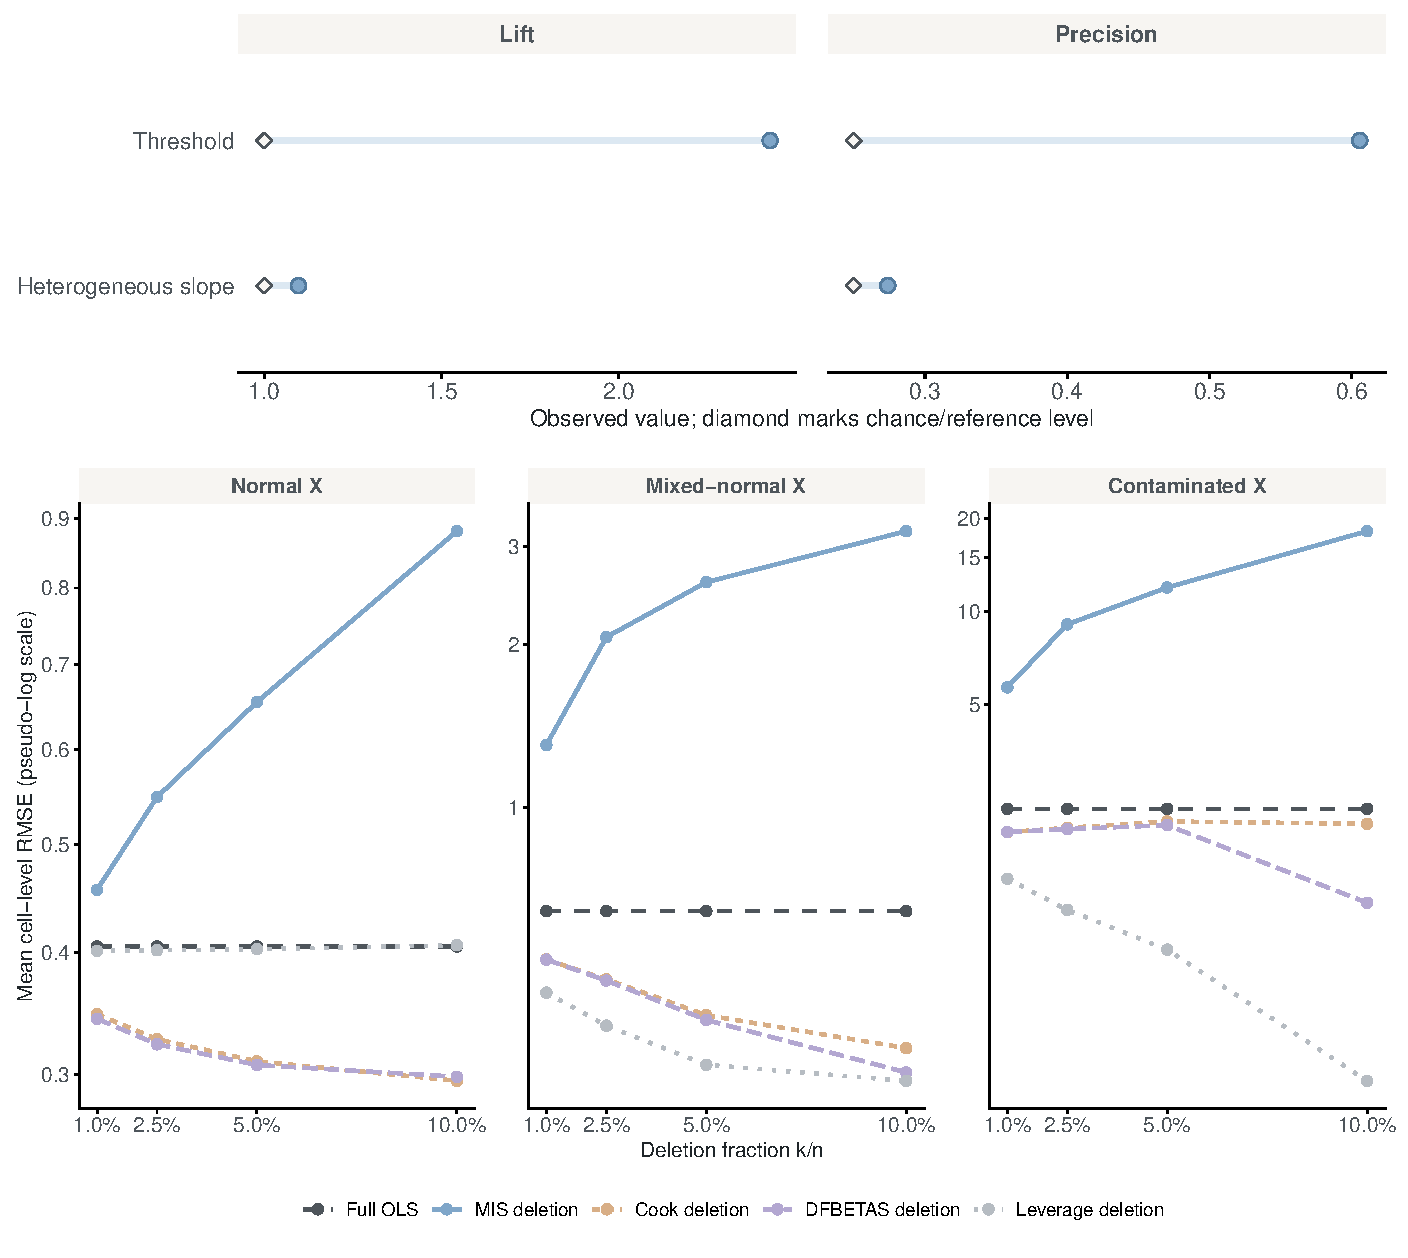
\includegraphics[width=\linewidth]{../../output/05_misspecification/figures/main/05_fig06_targeting_localisation.pdf}
	\caption{Mechanism-specific localisation and post-deletion coefficient error. The upper panels report localisation lift and precision for the heterogeneous-slope and threshold designs, with diamonds marking the corresponding chance/reference levels. The lower panels report mean cell-level coefficient RMSE for full-sample OLS and post-deletion OLS refits across fixed deletion fractions; predictor environments are displayed separately with different vertical scales.}
	\label{fig:05-targeting-localisation}
\end{figure}

The misspecification study establishes a second source of concentrated target-coefficient sensitivity. \autoref{fig:05-boundary-by-n} shows that its strength depends sharply on the form of the model departure, while \autoref{fig:05-targeting-localisation} shows that the composition of the selected set can vary independently of the overall sensitivity signal. Post-deletion coefficient error further gives localisation a diagnostic role within the maintained specification. Taken together, the three simulations show that concentrated target-coefficient sensitivity is mechanism dependent, that localisation and estimator stability are separate statistical objects, and that concentrated sensitivity can arise through both contamination and model misspecification. The empirical analysis next examines the magnitude and structure of this sensitivity across realised estimation samples.


\end{document}
